\chapter{Power management}
% Intro, cos'è il PM?

%TODO come è fatto un sistema HPC, def di nodo, etc.

Per svolgere al meglio il suo compito, un PowerStack deve interfacciarsi ad una serie di componenti HW e SW come: (i) sensori fisici, (ii) attuatori, (iii) sistema operativo e (iiii)applicazioni dell'utente. Successivamente, grazie a queste interfacce, viene monitorato lo stato di Processore, Temperatura e Tensione, impostando di conseguenza, (secondo delle politiche definite), il target di funzionamento. 

Oltre a queste metriche, il Power Management deve monitorare il consumo energetico delle tensioni dei binari dal Resource Manager (RM) e riceve dall'OS le richieste in termini di livello di prestazioni (Frequenza Obiettivo), budget energetico e caratteristiche del carico di lavoro da eseguire. La politica di gestione della potenza determina, in base a questi parametri, il miglior target di funzionamento in cui eseguire gli elementi di elaborazione, garantendo al contempo la stabilità termica, il budget energetico e i vincoli dell'applicazione. La gestione della potenza consente all'applicazione e al modello di programmazione in esecuzione di richiedere modifiche al target di funzionamento in modo asincrono per seguire le fasi dell'applicazione ed entrare in punti di funzionamento a basso consumo energetico durante le fasi limitate dall'I/O, dalla memoria e dalla comunicazione per aumentare l'efficienza energetica.


\section{Stato dell'arte}

% Come mostrato nella {Figura 1},
Il Power Management è collegato: (i) on-chip ai Power Management (gestendo il consumo energetico e le prestazioni degli elementi di elaborazione principali) e ai sensori (monitorando il processo, la temperatura e la tensione degli elementi di elaborazione principali); (ii) off-chip ai Moduli Regolatori di Tensione (VRM) che alimentano il chip, gli altri componenti a bordo e il Controller di Gestione della Scheda (BMC).

Questi componenti hardware vengono utilizzati per offrire un insieme di servizi in-band e out-of-band.

I servizi in-band vengono forniti alle applicazioni e ai sistemi operativi in esecuzione negli elementi di elaborazione del chip e sono composti da: (i) governor dedicati alla potenza e telemetria correlata alla potenza a livello di sistema operativo; (ii) un'interfaccia dedicata per consentire alle applicazioni e ai tempi di esecuzione del modello di programmazione di specificare suggerimenti e prescrizioni per la gestione della potenza; (iii) un'interfaccia dedicata al Sistema e alla Gestione delle Risorse per supportare il capping della potenza a livello di CPU e nodo, nonché per gestire il compromesso tra Throughput ed Efficienza Energetica. I servizi out-of-band vengono forniti all'amministratore di sistema e agli strumenti di gestione del sistema tramite il Controller di Gestione della Scheda (BMC). Questi servizi consistono nella telemetria di potenza out-of-band, nel capping di potenza a livello di sistema e nella affidabilità e assistenza.

\subsection{Servizi In-Band}
%\subsection{Interfacce SO}
Il Power Management condivide una regione di memoria interna con lo spazio degli indirizzi I/O degli elementi di elaborazione. Questa interfaccia consente all'OS di accedere periodicamente a un insieme di strutture dati di stato contenenti lo stato del Power Management, le statistiche e il consumo energetico dei diversi binari di tensione e componenti. Queste informazioni possono essere utilizzate e accessibili dalle applicazioni e dagli utenti per monitorare in modo dettagliato l'energia consumata dalle applicazioni, consentendo la consapevolezza energetica.

\subsection{Servizi Out-of-Band}
%\subsection{Board Management COntroller}
Oltre alla politica di gestione della potenza e ai servizi In-Band, il Power Management si interfaccia con il BMC per supportare servizi Out-of-Band. Questi includono la telemetria dettagliata sullo stato di potenza e prestazioni del chip, il Power Management a livello di chip e a livello di sistema e la segnalazione di errori e guasti nel chip e nei processi principali.

\subsection{Interfacce di alto livello}
%TODO


%Magari nella sezione dei problemi
Nel corso degli anni sono state sviluppati diversi software come parti di Power Management come \emph{Variorum} (LLNL), \emph{GEOPM} (Intel)\cite{GEOPM}, and \emph{HDEEM} (Atos)\cite{HDEEM}. Tutti questi strumenti rappresentano un tentativo di risolvere un problema specifico di Power Management e non un software globale di gestione dell'energia di sistemi HPC.
% Additionally, have been introduced predictive analysis and machine learning\cite{MLEC} algorithms. Predictive algorithms can predict load spikes and implement precautionary measures to lower consumption, while machine learning can fine-tune energy management strategies using historical and real-time data. Moreover, predictive algorithms often based on ML models are essential for estimating the workload sensitivity to a given power reduction or operating point selection. Indeed, it is essential for energy management and power management algorithm to reason on an implicit or explicit performance model.

% All these solutions represent attempts to tackle power management challenges, yet they display differing levels of compatibility. This lack highlights the urgent need for a comprehensive interoperability framework. These tools, though efficacious for specific use cases, often fail to cohesively integrate and cooperate due to varying interfaces and implementations.

\section{Componenti PowerStack}
Un power stack completo e interoperabile, deve essere composto da  attori che svolgono ruoli ben precisi. Tra questi i più importanti sono:
\begin{itemize}
    \item Workflow engine
    \item System Manager
    \item Job Manager
    \item Node Manager
    \item Monitor
\end{itemize}

Di seguito viene riportato uno schema\ref{fig:powerstackscheme} che mostra le interazioni tra i vari attori.
\begin{figure}[H]
    \centering
    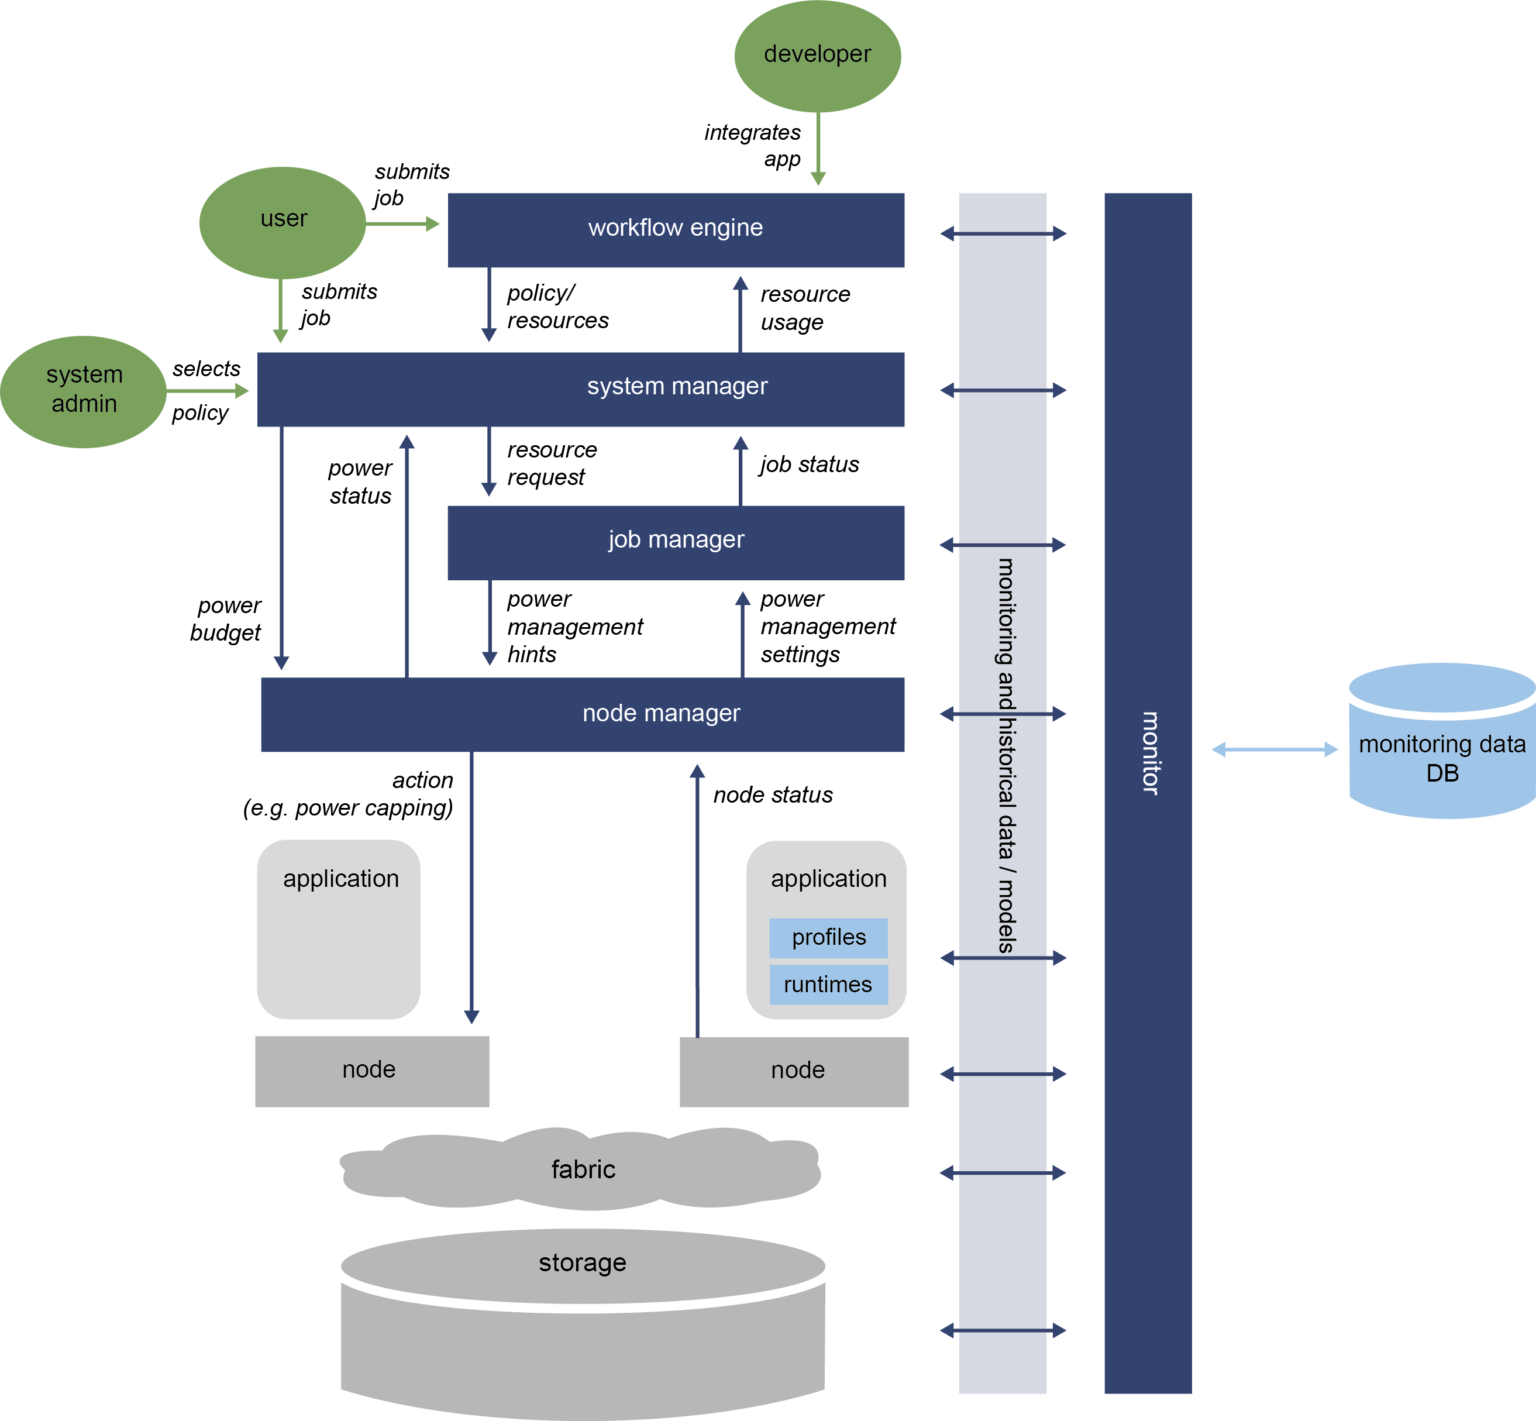
\includegraphics[width=\textwidth]{img/REGALE-Architecture-1536x1421.png} 
    \label{fig:powerstackscheme}
\end{figure}
\subsection{Workflow engine}
Il workflow engine analizza le dipendenze e le richieste di risorse di ogni workflow e decide dinamicamente come dividerlo negli specifici jobs che verranno assegnati al system-manager.

\subsection{Job schedulers}
Il job scheduler ha il compito di assegnare e condividere le risorse computazionali e fisice del sistema HPC, ai vari utenti che lo utilizzano. In particolare la serie di compiti che si trova a svolgere è il seguente L'utente schedula i jobs da svolgere in una o più code, definite dallo scheduler. Il Job scheduler esamina tutte le code e i job in esse contenute, e decide dinamicamente, quale sarà l'ordine di esecuzione, e il tempo massimo in cui viene assegnata una risorsa. Generalmente si cerca di ottimizzare alcune caratteristiche come il tempo di utilizzo del sistema oppure l'accesso veloce alle risorse per alcuni sottoinsiemi di jobs. Inoltre le code definite, possono avere diverse priorità o può essere ristretto l'accesso a soli alcuni utenti. 


\subsection{System Manager}
Riceve come input un insieme di jobs che devono essere schedulati all'interno del sistema, e in modo indicativo decide quando schedulare ogni job, su quale nodo, e con quale power budget. Successivamente vengono monitorati i dati relativi a potenza ed energia, e controlla di conseguenza i budget di potenza, e la \emph{user-fairness}

%To carry out its work, a job scheduler typically interacts with one or more resource managers. A resource manager is a piece of system software that has privileged ability to control various resources within a datacenter. These resources can include things such as the physical nodes that make up a highperformance computer's computational resources; disks, disk channels, or burst buffer hardware that comprise I/O resources; or network interfaces, network channels, or switches that comprise interconnect resources. For example, a job scheduler might use resource management software to configure the processing cores, memory, disk, and networking resources within one or more computational nodes in accordance with the requested resources for a specific batch job prior to launching that job onto the allocated computational nodes. Finally, in some cases, resource management software might have the ability to actuate pieces of the physical plant that are responsible for delivering electricity to the datacenter or cooling the datacenter

\subsection{Job Manager}
Il job manager decide i target delle manopole del Power Management, come (i) CPU power cap, (ii) CPU clock frequency oltre ad eseguire ottimizzazione del codice.

\subsection{Node Manager}
Il node manager fornisce accesso ai controlli e monitoraggio hardware a livello del nodo. Volendo permette anche di definire delle policy di power management. Ha infine lo scopo di preservare integrità, sicurezza del nodo sia in termini informatici che fisici.


\subsection{Monitor}

Il monitor è responsabile di collezionare tutte le metriche in-band e out-of-band che riguardando:
\begin{itemize}
    \item prestazioni
    \item Utilizzo di risorse
    \item Stato delle risorse
    \item Potenza
    \item Energia
\end{itemize}
Tutto questo deve essere fatto con il minor impatto possibile sul sistema dove sta agendo, collezionando, aggregando e analizzando le metriche e dove necessario, scambiandole ad altri attori.


% TODO:
% To ask andrea:
% Quali di questi componenti sono out-in band?